\documentclass[a4paper,11.5pt]{article}
\usepackage[textwidth=170mm, textheight=230mm, inner=20mm, top=20mm, bottom=30mm]{geometry}
\usepackage[normalem]{ulem}
\usepackage[utf8]{inputenc}
\usepackage[T1]{fontenc}
\PassOptionsToPackage{defaults=hu-min}{magyar.ldf}
\usepackage{pgfplots}
\pgfplotsset{compat=1.10}
\usepgfplotslibrary{fillbetween}
\usepackage[magyar]{babel}
\usepackage{amsmath, amsthm,amssymb,paralist,array, ellipsis, graphicx, float, bigints,tikz}
%\usepackage{marvosym}

\makeatletter
\renewcommand*{\mathellipsis}{%
	\mathinner{%
		\kern\ellipsisbeforegap%
		{\ldotp}\kern\ellipsisgap
		{\ldotp}\kern\ellipsisgap%
		{\ldotp}\kern\ellipsisaftergap%
	}%
}
\renewcommand*{\dotsb@}{%
	\mathinner{%
		\kern\ellipsisbeforegap%
		{\cdotp}\kern\ellipsisgap%
		{\cdotp}\kern\ellipsisgap%
		{\cdotp}\kern\ellipsisaftergap%
	}%
}
\renewcommand*{\@cdots}{%
	\mathinner{%
		\kern\ellipsisbeforegap%
		{\cdotp}\kern\ellipsisgap%
		{\cdotp}\kern\ellipsisgap%
		{\cdotp}\kern\ellipsisaftergap%
	}%
}
\renewcommand*{\ellipsis@default}{%
	\ellipsis@before
	\kern\ellipsisbeforegap
	.\kern\ellipsisgap
	.\kern\ellipsisgap
	.\kern\ellipsisgap
	\ellipsis@after\relax}
\renewcommand*{\ellipsis@centered}{%
	\ellipsis@before
	\kern\ellipsisbeforegap
	.\kern\ellipsisgap
	.\kern\ellipsisgap
	.\kern\ellipsisaftergap
	\ellipsis@after\relax}
\AtBeginDocument{%
	\DeclareRobustCommand*{\dots}{%
		\ifmmode\@xp\mdots@\else\@xp\textellipsis\fi}}
\def\ellipsisgap{.1em}
\def\ellipsisbeforegap{.05em}
\def\ellipsisaftergap{.05em}
\makeatother

\usepackage{hyperref}
\hypersetup{
	colorlinks = true	
}

\DeclareMathOperator{\Int}{int}
\DeclareMathOperator{\tg}{tg}
\DeclareMathOperator{\ctg}{ctg}
\DeclareMathOperator{\Th}{th}
\DeclareMathOperator{\sh}{sh}
\DeclareMathOperator{\ch}{ch}
\DeclareMathOperator{\arsh}{arsh}
\DeclareMathOperator{\arch}{arch}
\DeclareMathOperator{\arth}{arth}
\DeclareMathOperator{\arcth}{arcth}
\DeclareMathOperator{\grad}{grad}
\DeclareMathOperator{\arc}{arc}
\DeclareMathOperator{\arctg}{arc tg}
\DeclareMathOperator{\arcctg}{arc ctg}
\newcommand{\norm}[1]{\left\lVert#1\right\rVert}

\begin{document}
	%%%%%%%%%%%RÖVIDÍTÉSEK%%%%%%%%%%
	\setlength\parindent{0pt}
	\def\a{\textbf{a}}
	\def\b{\textbf{b}}
	\def\N{\hskip 10 true mm}
	\def\a{\textbf{a}}
	\def\b{\textbf{b}}
	\def\c{\textbf{c}}
	\def\d{\textbf{d}}
	\def\e{\textbf{e}}
	\def\gg{$\gamma$}
	\def\vi{\textbf{i}}
	\def\jj{\textbf{j}}
	\def\kk{\textbf{k}}
	\def\fh{\overrightarrow}
	\def\l{\lambda}
	\def\m{\mu}
	\def\v{\textbf{v}}
	\def\0{\textbf{0}}
	\def\s{\hspace{0.2mm}\vphantom{\beta}}
	\def\Z{\mathbb{Z}}
	\def\Q{\mathbb{Q}}
	\def\R{\mathbb{R}}
	\def\C{\mathbb{C}}
	\def\N{\mathbb{N}}
	\def\Rn{\mathbb{R}^{n}}
	\def\Ra{\overline{\mathbb{R}}}
	\def\sume{\displaystyle\sum_{n=1}^{+\infty}}
	\def\sumn{\displaystyle\sum_{n=0}^{+\infty}}
	\def\biz{\emph{Bizonyítás:\ }}
	\def\narrow{\underset{n\rightarrow+\infty}{\longrightarrow}}
	\def\limn{\displaystyle\lim_{n\to +\infty}}
	%	\def\definition{\textbf{Definíció:\ }}
	%	\def\theorem{\textbf{Tétel:\ }}
	%\def\note{\emph{Megjegyzés:\ }}
	%\def\example{\textbf{Példa:\ }} 
	
	\theoremstyle{definition}
	\newtheorem{theorem}{Tétel}[subsubsection] % reset theorem numbering for each chapter
	
	\theoremstyle{definition}
	\newtheorem{definition}[theorem]{Definíció} % definition numbers are dependent on theorem numbers
	\newtheorem{example}[theorem]{Példa} % same for example numbers
	\newtheorem{exercise}[theorem]{Házi feladat} % same for example numbers
	\newtheorem{note}[theorem]{Megjegyzés} % same for example numbers
	\newtheorem{task}[theorem]{Feladat} % same for example numbers
	\newtheorem{revision}[theorem]{Emlékeztető} % same for example numbers
	%%%%%%%%%%%%%%%%%%%%%%%%%%%%%%%%%
	\begin{center}
		{\LARGE\textbf{Analízis 3. A szakirány}}
		\smallskip
		
		{\Large Gyakorlati jegyzet}
		
		\smallskip
		13. óra.
	\end{center}
	A jegyzetet \textsc{Umann} Kristóf készítette \textsc{Filipp} Zoltán István gyakorlatán. (\today)
	\subsection{Egyenletes folytonosság}
	\begin{revision}
		(egyenletes folytonosság $\R^2$-en) Ha $f\in\R^2\to\R$, akkor $f$ egyenletesen folytonos egy $H\subset \mathcal{D}_f$ halmazon ($f\in EC(H))$, ha
		\[ \forall\varepsilon>0,\quad \exists\delta>0,\quad \forall(x,y),(a,b)\in H:\quad \norm{(x,y)-(a,b)}_{\R^2}<\delta:\quad |f(x,y)-f(a,b)|<\varepsilon \]
		\begin{figure}[H]
			\centering
			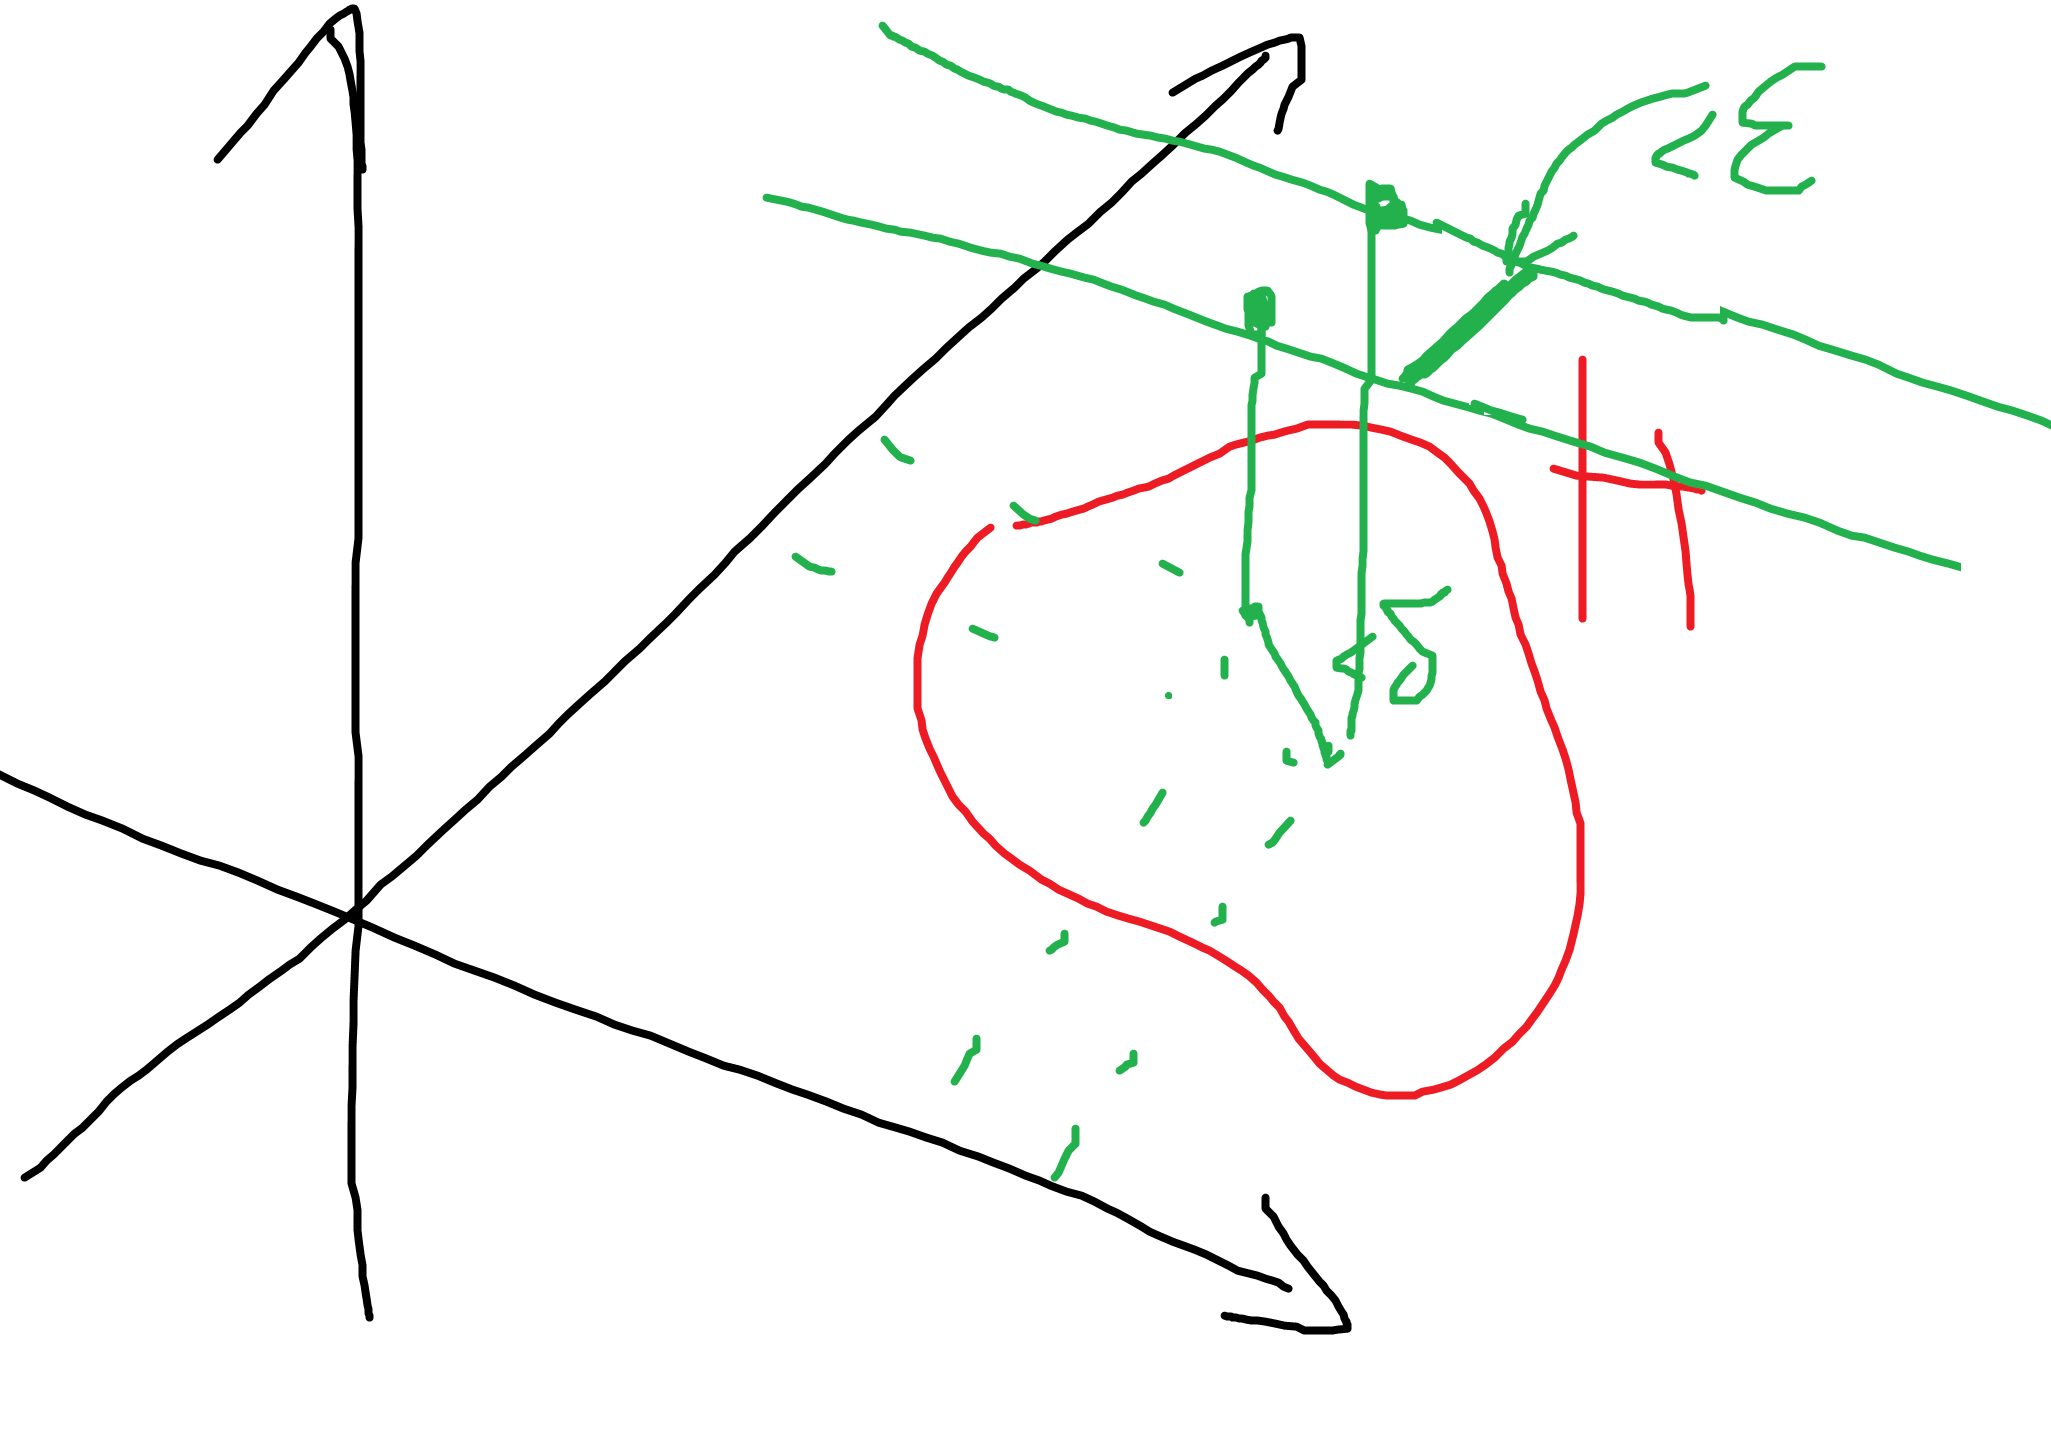
\includegraphics[height=4cm]{../2zh/kepek/52.png}
			\caption{}
		\end{figure}
	\end{revision}
	\begin{revision}
		Ha $f\in EC(H)\Rightarrow\quad f\in C(H)$.
	\end{revision}
	\begin{task}
		\[ f(x,y):=2x+3y-5\quad ((x,y)\in\R^2) \]
		Bizonyítsuk be, hogy egyenletesen folytonos!
		
		\smallskip
		\textit{Megoldás:} Sejtés: $f$ egyenletesen folytonos (értelemszerűen $\mathcal{D}_f=\R^2$-en).
		
		Ugyanis:
		\[ \varepsilon>0\quad \text{fix}\quad |f(x,y)-f(a,b)|=|2x+5y-5-(2a+3b-5)|=|2(x-a)+3(y-b)|\leq \]
		Cél lenne ezt felülről becsülni $\norm{(x,y)-(a,b)}$ valamilyen konstans szorosával. Ezt nem lehet minden példánál megcsinálni, azonban direkt bizonyításnál gyakran célravezető.
		\[ \leq2|x-a|+3|y-b|\overset{*}{\leq} 3|x-a|+3|y-b|=3\norm{x-a,y-b}_1=3\norm{(x,y)-(a,b)}_1<\varepsilon\quad \Leftrightarrow\quad \norm{(x,y)-(a,b)}_1<\frac{\varepsilon}{3}  \]
		Így:
		\[ \forall\varepsilon>0,\quad \exists\delta:=\frac{\varepsilon}{3},\quad \forall(x,y),(a,b)\in\R^2 : \norm{(x,y)-(a,b)}<\delta:\quad |f(x,y)-f(a,b)|\leq 3\norm{(x,y)-(a,b)}_1<3\frac{\varepsilon}{3}=\varepsilon  \]
		A korábban csillaggal jelölt résznél máshogy is becsülhetünk:
		\[ \leq 5\cdot\max\{ |x-a|;|y-b|\}=5\norm{(x,y)-(a,b)}_\infty<\varepsilon\quad \Leftrightarrow\quad \delta:=\frac{\varepsilon}{5}\quad \text{jó.} \]
		
	\end{task}
	\begin{note}
		Ha tekintsük a $z=3x+2y-5$ egyenletet, erről megállapítható hogy ez egy \textit{sík} egyenlete, ezt átrendezve megadható egy vektor ($n_s=(2,3,-1)$), melyre merőleges sík lesz az, melynek a fenti egyenlet megfeleltethető.
	\end{note}
	\begin{task}
		\[ f(x,y):=\sin\frac{\pi}{1-x^2-y^2} \quad ((x,y)\in D:=\{ (x,y)\in\R^2 \ | \ x^2+y^2<1 \}) \]
		
		
		\begin{figure}[H]
			\centering
			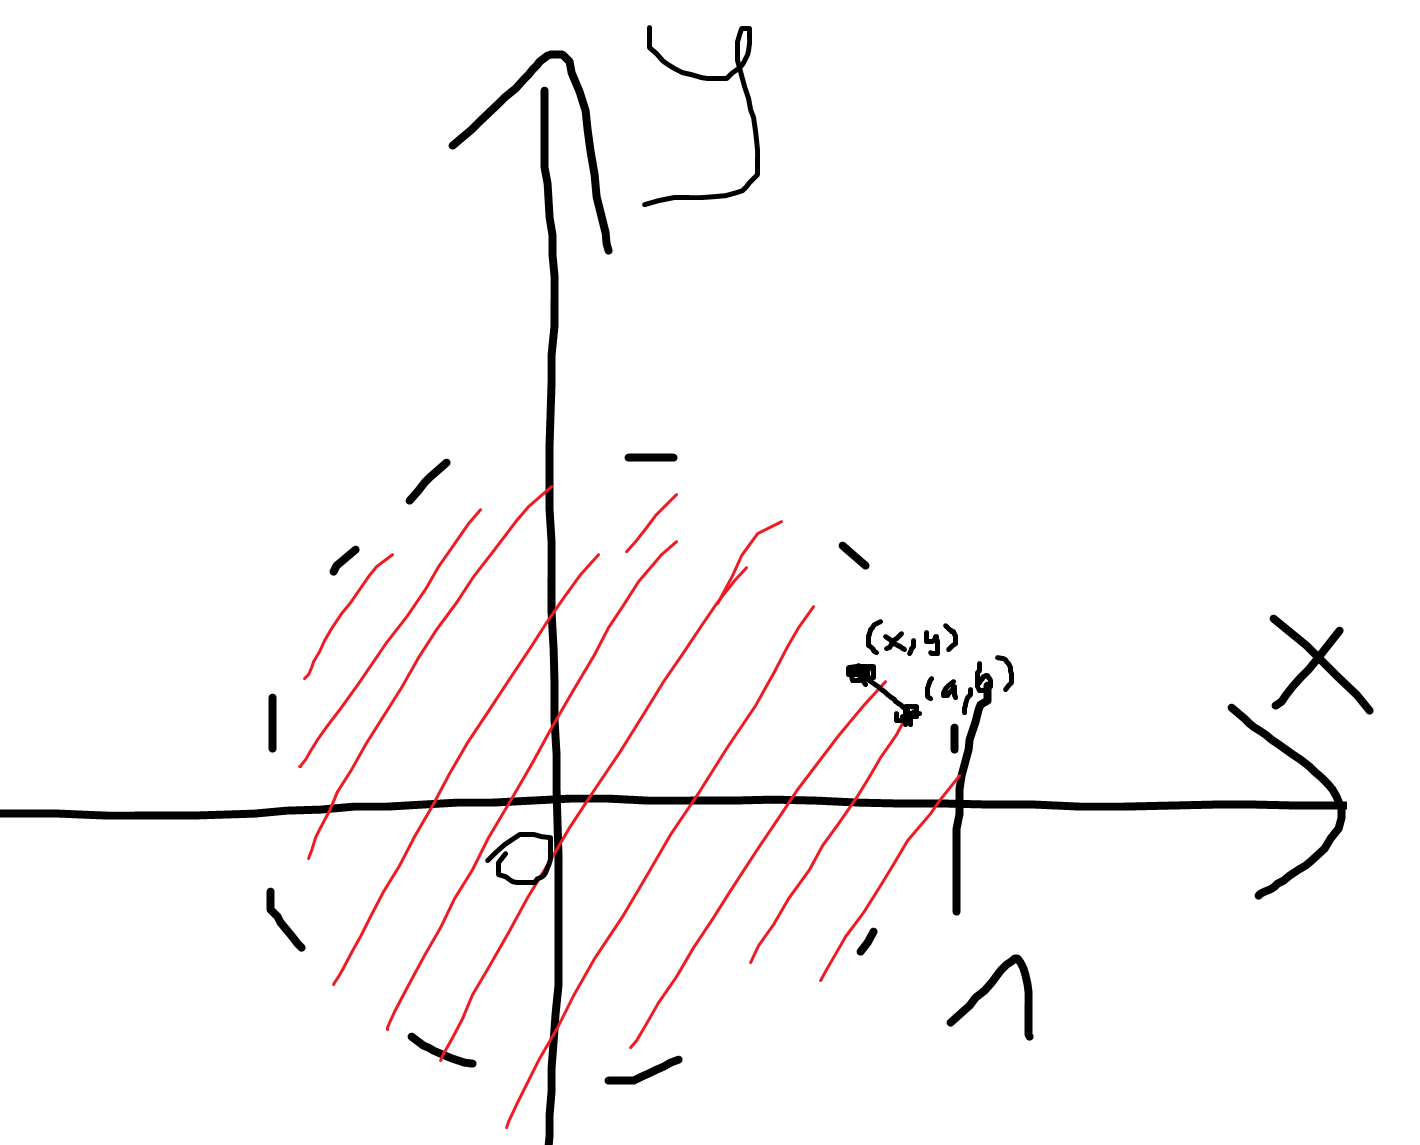
\includegraphics[height=4cm]{../2zh/kepek/53.png}
			\caption{Így néz ki az $f$ függvény értelmezési tartománya.}
		\end{figure}
		
		
		\textit{Megoldás:} Ki kéne alakítanunk egy sejtést, hogy vajon folytonos lesz-e ez a függvény. Érezhető, hogy problémás lesz a definíció, ha $(x^2+y^2)$ közelít 1-hez. Ez alapján
		
		\textit{Sejtés:} $f\notin EC(H)$, azaz
		\[ \exists\varepsilon>0:\quad \forall\delta>0,\quad \exists(x,y),(a,b)\in H:\quad \norm{(x,y)-(a,b)}_{\R^2}<\delta:\quad |f(x,y)-f(a,b)|\geq \varepsilon  \]
		Ennek a belátására egy új módszert fogunk alkalmazni. Ezt a módszert azonban függvények egyenletes folytonosságának \textit{bizonyítására} ne alkalmazzuk!
		
		Elég konstruálnunk olyan ($x_n,y_n$),$(a_n,b_n):\N\to H$ sorozatot, melyekre
		\[ \norm{(x_n,y_n)-(a_n,b_n)}_{\R^2}\to0\quad (\text{ha } n\to+\infty)\quad \text{és}\quad |f(x_n,y_n)-f(a_n,b_n)|\geq \varepsilon\quad \text{konstans} \] 
		\begin{center}
			\textit{,,Altassuk el az egyik változót!''}
			
			/Filipp/
		\end{center}
		\[ y=0\quad \text{mentén}\quad \Rightarrow\quad f(x,0)=\sin\frac{\pi}{1-x^2}\quad (x\in(-1,1)) \]
		Ezt ábrázolni se lenne nehéz, lényegében ez az $x$ tengelyen a $(-1,1)$ intervallum.
		
		Ötlet: adjuk meg az $(x_n),(a_n)$ sorozatokat úgy, hogy:
		\[ \sin\frac{\pi}{1-x_n^2}=1,\quad \sin\frac{\pi}{1-a_n^2}=0 \] 
		Ezzel ugyanis el tudnánk érni hogy az abszolút értékük különbsége $\varepsilon=1$ legyen mindig.
		
		Most szükségünk lesz egy olyan sorozatra, mely ezeknek meg is felel.
		\[ \Rightarrow\quad \frac{\pi}{1-x_n^2}=\frac{\pi}{2}+2n\pi \quad \Rightarrow\quad 1-x_n^2=\overbrace{\frac{1}{\frac{1}{2}+2n}}^{\in(0,1)\subset(-1,1)}\quad \Rightarrow\quad x_n:=\sqrt{1-\frac{1}{\frac{1}{2}+2n}}\quad (1\leq n\in\N)  \]
		Ezzel sikeresen elértük hogy az $(x_n)$ a (-1,1) intervallum vegyen fel értékeket.
		\[ \frac{\pi}{1-a_n^2}=2n\pi\quad \Rightarrow\quad \frac{1}{2n}=1-a_n^2\quad \Rightarrow\quad a_n:=\sqrt{1-\frac{1}{2n}}\quad (1\leq n\in\N) \]
		Ezzel elértük hogy $(x_n),(a_n):\N\to(-1,1)\checkmark$. Ekkor:
		\[ \norm{(x_n,0)-(a_n,0)}_1=\norm{(x_n-a_n,0)}_1=|x_n-a_n|=\]
		\[=\left|\sqrt{1-\frac{1}{\frac{1}{2}+2n}}-\sqrt{1-\frac{1}{2n}}\right|\to|\sqrt{1}-\sqrt{1}|=0\checkmark\quad (\text{ha } n\to+\infty )\quad \text{és}\quad |f(x_n,0)-f(a_n,0)|=1-0=:\varepsilon \]
		Összefoglalva:
		\[ \exists\varepsilon:=1\quad \forall\delta>0\quad \exists1\leq n_0\in\N\quad \text{és}\quad (x_{n_0},0)(a_{n_0},0)\in \mathcal{D}:\quad \norm{(x_{n_0})-(a_{n_0},0)}_1<\delta\]
		\[ |f(x_{n_0},0)-f(a_{n_0},0)|=1 \geq\varepsilon=1\quad \Rightarrow\quad f\notin EC(\mathcal{D}) \]
		
	\end{task}
	\begin{task}
		\[ f(x,y):=\frac{\sin\left(x^2+y^2+e^{x^4}\right)}{1+\arctg^2x}\quad ((x,y)\in\R^2) \]
		,,Lőjünk ki egy változót'', ezzel egyszerűsítve a függvényt.
		\[ x=0\quad \text{mentén}\quad f(0,y)=\sin(1+y^2)\quad (y\in\R) \]
		Lássuk be, hogy ez nem egyenletesen folytonos!
		
		\begin{figure}[H]
			\centering
			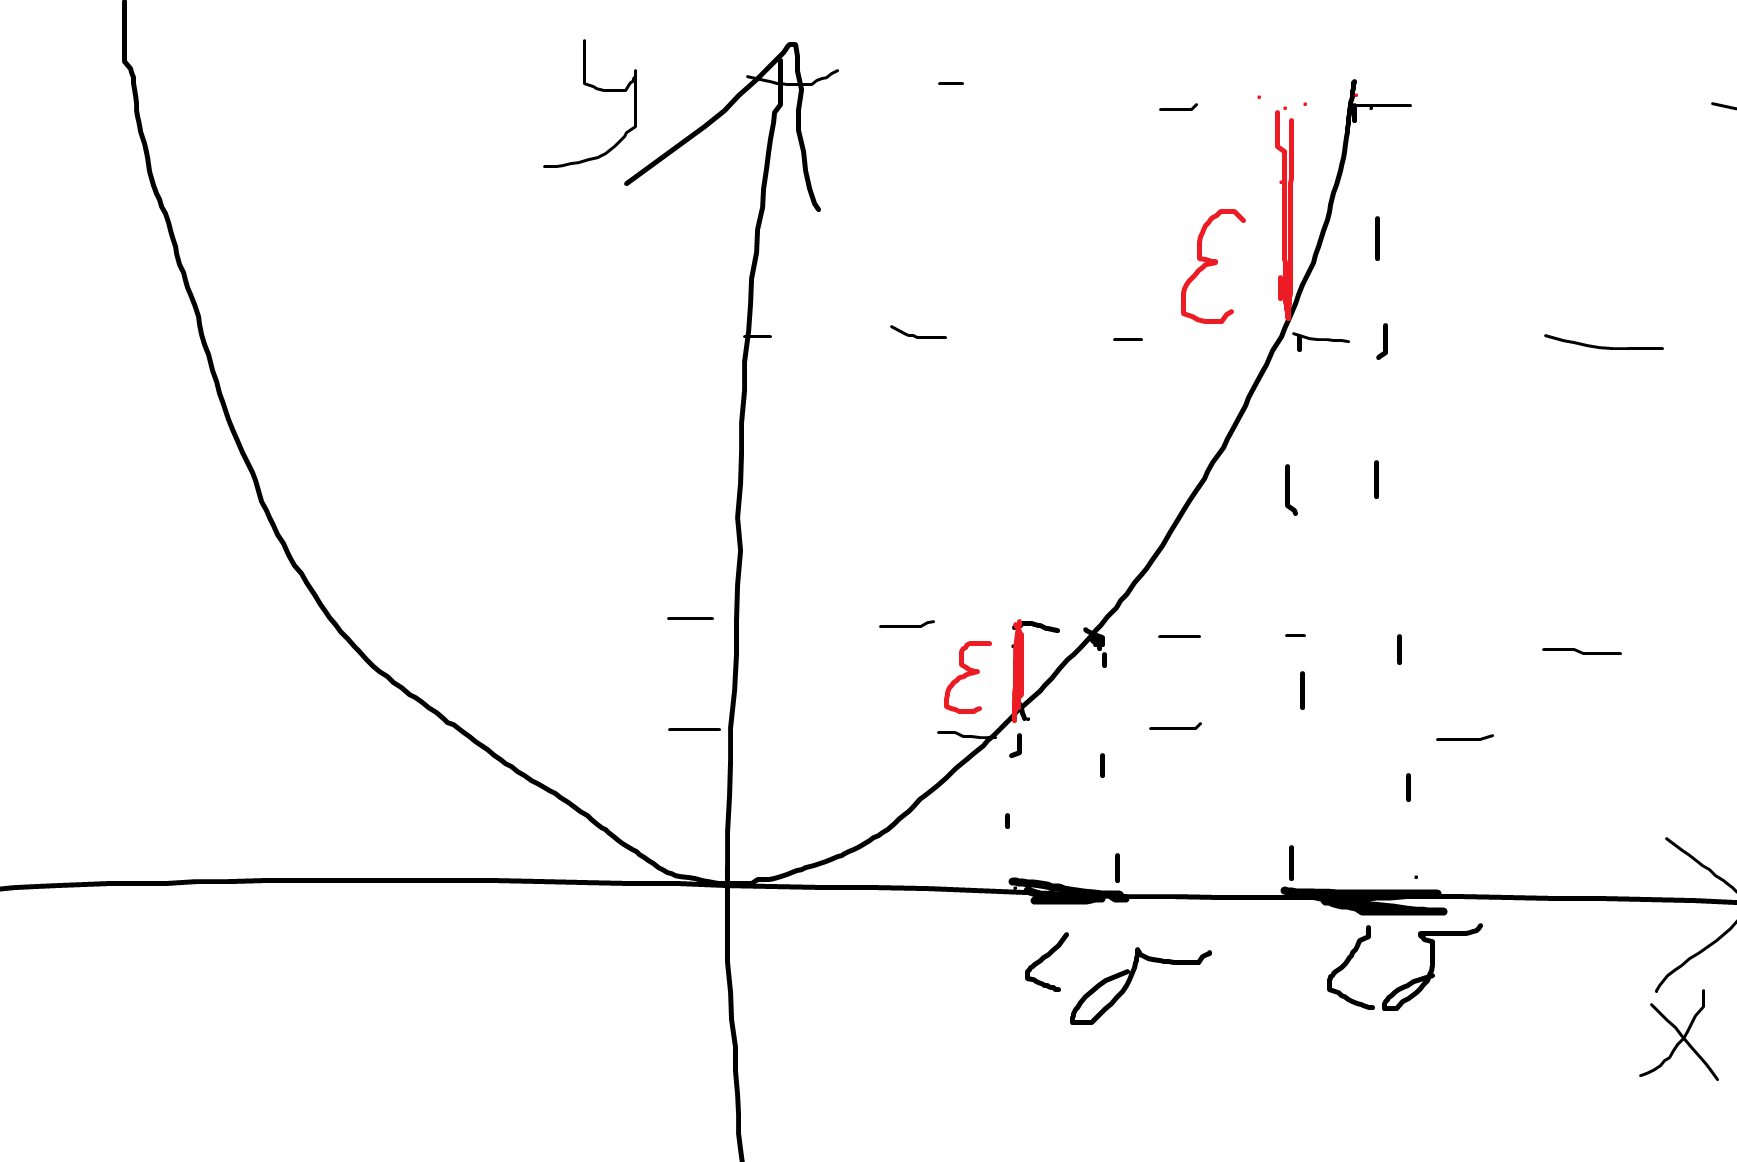
\includegraphics[height=4cm]{../2zh/kepek/54.png}
			\caption{Az $f(x)=x^2$ fv. nem egyenletesen folytonos.}
		\end{figure}
		
		\textit{Sejtés:} $f\notin EC(\R^2)$.
		
		\textit{Bizonyítás:} Legyen $(y_n),(b_n):\N\to\R$ olyanok, hogy:
		\[ \sin(y_n^2+1)=1,\quad \sin(b_n^2+1)=0 \]
		Ekkor:
		\[ y_n^2+1=\frac{\pi}{2}+2n\pi,\quad y_n:=\sqrt{\frac{\pi}{2}-1+2n\pi}\to+\infty\quad (\text{ha }n\to\infty) \]
		Valamint
		\[ b_n^2+1=2n\pi\Rightarrow\quad b_n:=\sqrt{2n\pi-1}\to+\infty,\quad (\text{ha } n\to\infty)\quad (1\leq n\in\N) \]
		Tehát:
		\[ \norm{(0,y_n)-(0,b_n)}_1=\left|\sqrt{\frac{\pi}{2}-1+2n\pi}-\sqrt{2n\pi-1}\right|=\frac{\frac{\pi}{2}}{\sqrt{\frac{\pi}{2}-1+2n\pi}+\sqrt{2n\pi-1}}\to0\quad (\text{ha }n\to+\infty) \]
		\[ |f(0,y_n)-f(0,b_n)|=|1-0|=1 \]
		Összefoglalva:
		\[ \exists\varepsilon:=1\quad \forall>0\quad \exists n_0\in\N:\quad (0,y_{n_0}),(0,b_{n_0})\in\mathcal{D}_f:\quad \norm{(0,y_{n_0})-f(0,b_{n_0})}|=1\geq\varepsilon:=1 \]
		$\Rightarrow\quad f\notin EC(\R^2)$.
	\end{task}
	\begin{note}
		\[ f(x,y)=\sin\frac{\pi}{1-x^2-y^2};\quad (x,y)\in\overline{k_R(0,0)}=\{ (x,y)\in\R^2\ | \ x^2+y^2\leq \R^2 \}\quad (\forall 0<R<1)\quad \overset{\text{Heine.}}{\Rightarrow}\quad f\in EC(D_R), \]
		ahol a felülvonás lezártat jelent.
		\begin{figure}[H]
			\centering
			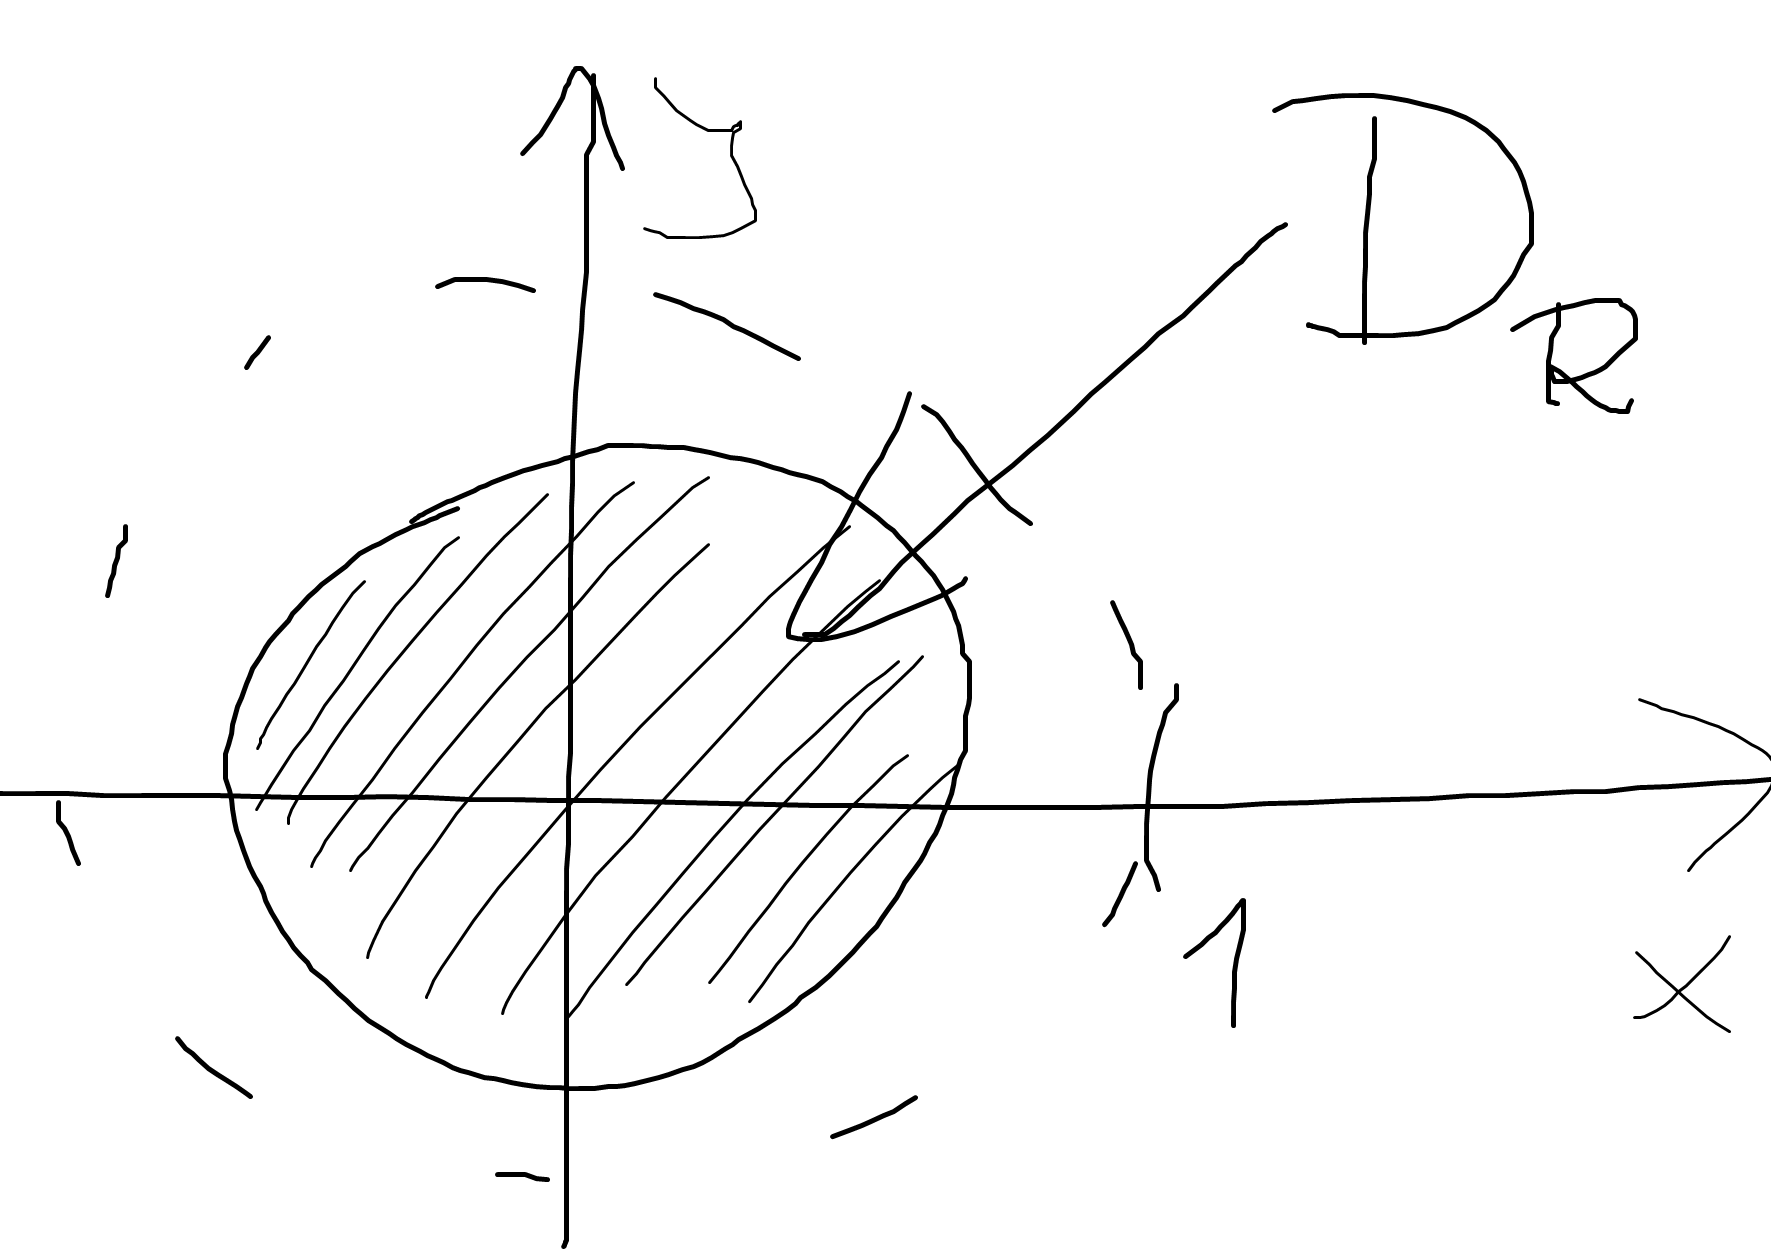
\includegraphics[height=4cm]{../2zh/kepek/55.png}
			\caption{$D_R$ egy zárt körlap}
		\end{figure}
	\end{note}
	\begin{task}
		\[ f(x,y):=\sqrt{x^2+y^2}\quad ((x,y)\in\R^2) \]
		Igaz-e hogy $f\in EC$?
		
		\textit{Megoldás:} 
		\[ \varepsilon>0\quad \text{fix},\quad |f(x,y)-f(a,b)|=|\sqrt{x^2+y^2}-\sqrt{a^2+b^2}|\leq \]
		A cél ismét egy felső becslés megadása. Ha ezt direkt módszerrel próbálnánk, elég nehezen adná magát.
		
		Ötlet: $f(x,y):=\norm{(x,y)}_2$
		
		Tétel: Legyen ($X,\norm{\cdot}$) normált tér,
		\[ \Rightarrow\quad f(x,y):=\norm{x}\quad (x\in X) \]
		
		Ekkor:
		\[ |f(x)-f(t)|=\big|\norm{x}-\norm{t}\big|\overset{*}{\leq}\norm{x-t}<\varepsilon\quad \Leftrightarrow\quad \delta:=\varepsilon\quad \text{jó.} \]
		A kicsillagozott résznél lehet az átalakítás nem triviális, a kifejezés helyessége mögött ez áll:
		\begin{align*}
			\norm{x}=\norm{(x-t)+t}\leq\norm{x-t}+\norm{t}\quad& \Leftrightarrow\quad \norm{x}-\norm{t}\leq\norm{x-t}\\
			\norm{t}=\norm{(t-x)+x}\leq\norm{t-x}+\norm{x}\quad& \Leftrightarrow\quad \norm{t}-\norm{x}\leq\norm{t-x}\\
			\Rightarrow\quad -\norm{x-t}\leq\norm{x}-\norm{t}\leq\norm{x-t}\quad& \Leftrightarrow\quad \big|\norm{x}-\norm{t}\big|\leq \norm{x-t}
			%TODO finish
		\end{align*}
		De:
		\[ \left|\sqrt{x^2+y^2}-\sqrt{a^2+b^2}\right|=\frac{\left|\sqrt{x^2+y^2}-\sqrt{a^2+b^2}\right|}{\sqrt{x^2+y^2}-\sqrt{a^2+b^2}}\leq|x-a|\frac{|x+a|}{\sqrt{x^2+y^2}-\sqrt{a^2+b^2}}+|y-b|\frac{y+b}{\sqrt{x^2+y^2}-\sqrt{a^2+b^2}}= \]
		\[ = |x-a|\frac{|x|+|a|}{\sqrt{x^2 + a}^2}+|y-b|\frac{|y|+|b|}{\sqrt{y^2+b}^2}=|x-a|+|y-b|=\norm{(x,y)-(a,b)}_1 \] 
	\end{task}
	
	\bigskip
	Óriási köszönet \textsc{Qian} Líviának és \textsc{Hoang} Lászlónak a jegyzet javításáért, és természetesen \textsc{Filipp} Zoltánnak, aki fantasztikus gyakorlatot tartott a félév folyamán.
\end{document}